% Created by tikzDevice version 0.10.1 on 2016-04-22 17:11:55
% !TEX encoding = UTF-8 Unicode
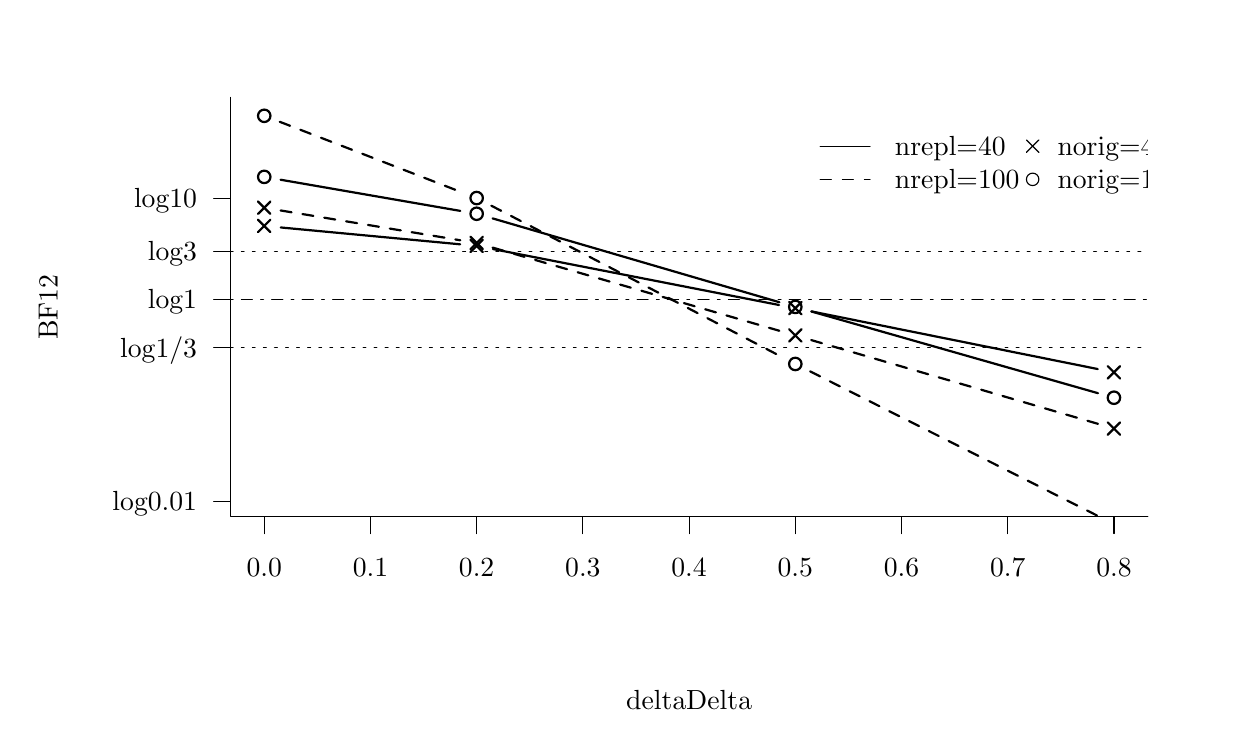
\begin{tikzpicture}[x=1pt,y=1pt]
\definecolor{fillColor}{RGB}{255,255,255}
\path[use as bounding box,fill=fillColor,fill opacity=0.00] (0,0) rectangle (430.00,250.00);
\begin{scope}
\path[clip] ( 73.20, 73.20) rectangle (404.80,224.80);
\definecolor{drawColor}{RGB}{0,0,0}

\path[draw=drawColor,line width= 0.8pt,line join=round,line cap=round] ( 91.46,177.80) -- (156.27,171.72);

\path[draw=drawColor,line width= 0.8pt,line join=round,line cap=round] (168.13,170.00) -- (271.49,149.79);

\path[draw=drawColor,line width= 0.8pt,line join=round,line cap=round] (283.26,147.46) -- (386.64,126.65);

\path[draw=drawColor,line width= 0.8pt,line join=round,line cap=round] ( 83.23,176.11) -- ( 87.73,180.61);

\path[draw=drawColor,line width= 0.8pt,line join=round,line cap=round] ( 83.23,180.61) -- ( 87.73,176.11);

\path[draw=drawColor,line width= 0.8pt,line join=round,line cap=round] (159.99,168.90) -- (164.49,173.40);

\path[draw=drawColor,line width= 0.8pt,line join=round,line cap=round] (159.99,173.40) -- (164.49,168.90);

\path[draw=drawColor,line width= 0.8pt,line join=round,line cap=round] (275.13,146.39) -- (279.63,150.89);

\path[draw=drawColor,line width= 0.8pt,line join=round,line cap=round] (275.13,150.89) -- (279.63,146.39);

\path[draw=drawColor,line width= 0.8pt,line join=round,line cap=round] (390.27,123.22) -- (394.77,127.72);

\path[draw=drawColor,line width= 0.8pt,line join=round,line cap=round] (390.27,127.72) -- (394.77,123.22);
\end{scope}
\begin{scope}
\path[clip] (  0.00,  0.00) rectangle (430.00,250.00);
\definecolor{drawColor}{RGB}{0,0,0}

\path[draw=drawColor,line width= 0.4pt,line join=round,line cap=round] ( 73.20,224.80) --
	( 73.20, 73.20) --
	(404.80, 73.20);
\end{scope}
\begin{scope}
\path[clip] (  0.00,  0.00) rectangle (430.00,250.00);
\definecolor{drawColor}{RGB}{0,0,0}

\node[text=drawColor,anchor=base,inner sep=0pt, outer sep=0pt, scale=  1.00] at (239.00,  3.60) {deltaDelta};

\node[text=drawColor,rotate= 90.00,anchor=base,inner sep=0pt, outer sep=0pt, scale=  1.00] at ( 10.80,149.00) {BF12};
\end{scope}
\begin{scope}
\path[clip] ( 73.20, 73.20) rectangle (404.80,224.80);
\definecolor{drawColor}{RGB}{0,0,0}

\path[draw=drawColor,line width= 0.8pt,dash pattern=on 4pt off 4pt ,line join=round,line cap=round] ( 91.40,183.95) -- (156.32,173.18);

\path[draw=drawColor,line width= 0.8pt,dash pattern=on 4pt off 4pt ,line join=round,line cap=round] (168.00,170.53) -- (271.62,140.47);

\path[draw=drawColor,line width= 0.8pt,dash pattern=on 4pt off 4pt ,line join=round,line cap=round] (283.14,137.11) -- (386.76,106.84);

\path[draw=drawColor,line width= 0.8pt,line join=round,line cap=round] ( 83.23,182.68) -- ( 87.73,187.18);

\path[draw=drawColor,line width= 0.8pt,line join=round,line cap=round] ( 83.23,187.18) -- ( 87.73,182.68);

\path[draw=drawColor,line width= 0.8pt,line join=round,line cap=round] (159.99,169.95) -- (164.49,174.45);

\path[draw=drawColor,line width= 0.8pt,line join=round,line cap=round] (159.99,174.45) -- (164.49,169.95);

\path[draw=drawColor,line width= 0.8pt,line join=round,line cap=round] (275.13,136.55) -- (279.63,141.05);

\path[draw=drawColor,line width= 0.8pt,line join=round,line cap=round] (275.13,141.05) -- (279.63,136.55);

\path[draw=drawColor,line width= 0.8pt,line join=round,line cap=round] (390.27,102.90) -- (394.77,107.40);

\path[draw=drawColor,line width= 0.8pt,line join=round,line cap=round] (390.27,107.40) -- (394.77,102.90);

\path[draw=drawColor,line width= 0.8pt,line join=round,line cap=round] ( 91.39,195.05) -- (156.33,183.79);

\path[draw=drawColor,line width= 0.8pt,line join=round,line cap=round] (168.00,181.08) -- (271.62,150.79);

\path[draw=drawColor,line width= 0.8pt,line join=round,line cap=round] (283.15,147.46) -- (386.75,117.92);

\path[draw=drawColor,line width= 0.8pt,line join=round,line cap=round] ( 85.48,196.08) circle (  2.25);

\path[draw=drawColor,line width= 0.8pt,line join=round,line cap=round] (162.24,182.76) circle (  2.25);

\path[draw=drawColor,line width= 0.8pt,line join=round,line cap=round] (277.38,149.10) circle (  2.25);

\path[draw=drawColor,line width= 0.8pt,line join=round,line cap=round] (392.52,116.28) circle (  2.25);

\path[draw=drawColor,line width= 0.8pt,dash pattern=on 4pt off 4pt ,line join=round,line cap=round] ( 91.08,215.99) -- (156.65,190.59);

\path[draw=drawColor,line width= 0.8pt,dash pattern=on 4pt off 4pt ,line join=round,line cap=round] (167.56,185.66) -- (272.06,131.25);

\path[draw=drawColor,line width= 0.8pt,dash pattern=on 4pt off 4pt ,line join=round,line cap=round] (282.74,125.79) -- (387.16, 73.34);

\path[draw=drawColor,line width= 0.8pt,line join=round,line cap=round] ( 85.48,218.15) circle (  2.25);

\path[draw=drawColor,line width= 0.8pt,line join=round,line cap=round] (162.24,188.43) circle (  2.25);

\path[draw=drawColor,line width= 0.8pt,line join=round,line cap=round] (277.38,128.48) circle (  2.25);

\path[draw=drawColor,line width= 0.8pt,line join=round,line cap=round] (392.52, 70.64) circle (  2.25);

\path[] (277.38,219.19) rectangle (362.90,183.19);

\path[draw=drawColor,line width= 0.4pt,line join=round,line cap=round] (286.38,207.19) -- (304.38,207.19);

\path[draw=drawColor,line width= 0.4pt,dash pattern=on 4pt off 4pt ,line join=round,line cap=round] (286.38,195.19) -- (304.38,195.19);

\node[text=drawColor,anchor=base west,inner sep=0pt, outer sep=0pt, scale=  1.00] at (313.38,203.74) {nrepl=40};

\node[text=drawColor,anchor=base west,inner sep=0pt, outer sep=0pt, scale=  1.00] at (313.38,191.74) {nrepl=100};

\path[] (354.14,219.19) rectangle (421.66,183.19);

\path[draw=drawColor,line width= 0.4pt,line join=round,line cap=round] (360.89,204.94) -- (365.39,209.44);

\path[draw=drawColor,line width= 0.4pt,line join=round,line cap=round] (360.89,209.44) -- (365.39,204.94);

\path[draw=drawColor,line width= 0.4pt,line join=round,line cap=round] (363.14,195.19) circle (  2.25);

\node[text=drawColor,anchor=base west,inner sep=0pt, outer sep=0pt, scale=  1.00] at (372.14,203.74) {norig=40};

\node[text=drawColor,anchor=base west,inner sep=0pt, outer sep=0pt, scale=  1.00] at (372.14,191.74) {norig=100};
\end{scope}
\begin{scope}
\path[clip] (  0.00,  0.00) rectangle (430.00,250.00);
\definecolor{drawColor}{RGB}{0,0,0}

\path[draw=drawColor,line width= 0.4pt,line join=round,line cap=round] ( 85.48, 73.20) -- (392.52, 73.20);

\path[draw=drawColor,line width= 0.4pt,line join=round,line cap=round] ( 85.48, 73.20) -- ( 85.48, 67.20);

\path[draw=drawColor,line width= 0.4pt,line join=round,line cap=round] (123.86, 73.20) -- (123.86, 67.20);

\path[draw=drawColor,line width= 0.4pt,line join=round,line cap=round] (162.24, 73.20) -- (162.24, 67.20);

\path[draw=drawColor,line width= 0.4pt,line join=round,line cap=round] (200.62, 73.20) -- (200.62, 67.20);

\path[draw=drawColor,line width= 0.4pt,line join=round,line cap=round] (239.00, 73.20) -- (239.00, 67.20);

\path[draw=drawColor,line width= 0.4pt,line join=round,line cap=round] (277.38, 73.20) -- (277.38, 67.20);

\path[draw=drawColor,line width= 0.4pt,line join=round,line cap=round] (315.76, 73.20) -- (315.76, 67.20);

\path[draw=drawColor,line width= 0.4pt,line join=round,line cap=round] (354.14, 73.20) -- (354.14, 67.20);

\path[draw=drawColor,line width= 0.4pt,line join=round,line cap=round] (392.52, 73.20) -- (392.52, 67.20);

\node[text=drawColor,anchor=base,inner sep=0pt, outer sep=0pt, scale=  1.00] at ( 85.48, 51.60) {0.0};

\node[text=drawColor,anchor=base,inner sep=0pt, outer sep=0pt, scale=  1.00] at (123.86, 51.60) {0.1};

\node[text=drawColor,anchor=base,inner sep=0pt, outer sep=0pt, scale=  1.00] at (162.24, 51.60) {0.2};

\node[text=drawColor,anchor=base,inner sep=0pt, outer sep=0pt, scale=  1.00] at (200.62, 51.60) {0.3};

\node[text=drawColor,anchor=base,inner sep=0pt, outer sep=0pt, scale=  1.00] at (239.00, 51.60) {0.4};

\node[text=drawColor,anchor=base,inner sep=0pt, outer sep=0pt, scale=  1.00] at (277.38, 51.60) {0.5};

\node[text=drawColor,anchor=base,inner sep=0pt, outer sep=0pt, scale=  1.00] at (315.76, 51.60) {0.6};

\node[text=drawColor,anchor=base,inner sep=0pt, outer sep=0pt, scale=  1.00] at (354.14, 51.60) {0.7};

\node[text=drawColor,anchor=base,inner sep=0pt, outer sep=0pt, scale=  1.00] at (392.52, 51.60) {0.8};

\path[draw=drawColor,line width= 0.4pt,line join=round,line cap=round] ( 73.20, 78.81) -- ( 73.20,188.33);

\path[draw=drawColor,line width= 0.4pt,line join=round,line cap=round] ( 73.20, 78.81) -- ( 67.20, 78.81);

\path[draw=drawColor,line width= 0.4pt,line join=round,line cap=round] ( 73.20,134.41) -- ( 67.20,134.41);

\path[draw=drawColor,line width= 0.4pt,line join=round,line cap=round] ( 73.20,151.83) -- ( 67.20,151.83);

\path[draw=drawColor,line width= 0.4pt,line join=round,line cap=round] ( 73.20,169.25) -- ( 67.20,169.25);

\path[draw=drawColor,line width= 0.4pt,line join=round,line cap=round] ( 73.20,188.33) -- ( 67.20,188.33);

\node[text=drawColor,anchor=base east,inner sep=0pt, outer sep=0pt, scale=  1.00] at ( 61.20, 75.37) {log0.01};

\node[text=drawColor,anchor=base east,inner sep=0pt, outer sep=0pt, scale=  1.00] at ( 61.20,130.97) {log1/3};

\node[text=drawColor,anchor=base east,inner sep=0pt, outer sep=0pt, scale=  1.00] at ( 61.20,148.38) {log1};

\node[text=drawColor,anchor=base east,inner sep=0pt, outer sep=0pt, scale=  1.00] at ( 61.20,165.80) {log3};

\node[text=drawColor,anchor=base east,inner sep=0pt, outer sep=0pt, scale=  1.00] at ( 61.20,184.89) {log10};
\end{scope}
\begin{scope}
\path[clip] ( 73.20, 73.20) rectangle (404.80,224.80);
\definecolor{drawColor}{RGB}{0,0,0}

\path[draw=drawColor,line width= 0.4pt,dash pattern=on 1pt off 3pt on 4pt off 3pt ,line join=round,line cap=round] ( 73.20,151.83) -- (404.80,151.83);

\path[draw=drawColor,line width= 0.4pt,dash pattern=on 1pt off 3pt ,line join=round,line cap=round] ( 73.20,134.41) -- (404.80,134.41);

\path[draw=drawColor,line width= 0.4pt,dash pattern=on 1pt off 3pt ,line join=round,line cap=round] ( 73.20,169.25) -- (404.80,169.25);
\end{scope}
\end{tikzpicture}
